% =====================================================================
% VERSION INSTITUT A 150 PAGES : demonstrations et complements sur le socle de valeurs extremes.
% Reprise de materiel_complementaire/15_demonstrations.tex et des sections « Hill contre maximum de
% vraisemblance » et « seuil de la calibration » de 21_complements_corps.tex, reecrites en phrases
% courtes. Les nombres, formules et etiquettes sont ceux de l'original, a une exception : la
% matrice d'information de Fisher de la GPD, ou le facteur 1/(1+xi) manquait a l'original, qui
% n'etait pas coherent avec l'inverse qu'il donnait (corrige ici, resultat final inchange).
% Lue par main_institut_150.tex seul.
% =====================================================================

\chapter{Démonstrations et compléments sur la théorie des valeurs extrêmes}
\label{ann:evt}

Les preuves de stabilité de la cascade et de la propriété de branchement sont à l'annexe~\ref{ann:cascade}.
Les preuves complètes des théorèmes de valeurs extrêmes sont données par \citet{Embrechts1997} ;
nous n'en rappelons que les arguments.
% HARNAIS-HORS-SCRIPT: sections de demonstrations : les nombres y sont des constantes d'enonce
% (bornes, exposants), aucun n'est un resultat calcule par le pipeline.

\section{Théorème de Fisher-Tippett-Gnedenko}
\label{soc:ann:ftg}

La loi limite $H$ des maxima normalisés est max-stable. Pour tout $t>0$, on a $H^t(x)=H(a_tx+b_t)$,
par passage à la limite des maxima de blocs pour les entiers, puis extension en $t$. En posant
$g(x)=-\ln H(x)$, la max-stabilité devient l'équation fonctionnelle $t\,g(x)=g(a_tx+b_t)$. Sa résolution,
par la classification des lois max-stables, donne, après normalisation, $g(x)=(1+\xi x)^{-1/\xi}$
sur $1+\xi x>0$, avec $g(x)=e^{-x}$ si $\xi=0$. C'est la famille $H_\xi$.

Le domaine d'attraction se lit ensuite sur la queue de $F$. On a $F\in\mathrm{DA}(H_\xi)$ avec $\xi>0$ si et
seulement si $\bar F$ est à variation régulière d'indice $-1/\xi$, soit $\bar F(tx)/\bar F(x)\to t^{-1/\xi}$.
Les lois lognormale et gamma relèvent du cas $\xi=0$ (Gumbel). Un support borné ne suffit pas à
imposer $\xi<0$ : le domaine Weibull requiert une condition de variation régulière à la borne.

\section{Théorème de Pickands-Balkema-de Haan}
\label{soc:ann:balkema}

Pour $F\in\mathrm{DA}(H_\xi)$, il existe une fonction positive $a(\cdot)$ telle que, pour $y\ge0$ tel que $1+\xi y>0$,
$\lim_{u\to x_F}\bar F(u+y\,a(u))/\bar F(u)=(1+\xi y)^{-1/\xi}$. Le quotient vaut
$\Prob(X>u+ya(u)\mid X>u)=1-F_u(y\,a(u))$, et sa limite est la survie $\bar G_{\xi,1}(y)$ de la GPD. En
posant $\sigma(u)=a(u)$, on obtient une approximation GPD des excès ; pour $\xi=0$, la survie limite vaut $e^{-y}$.

Le théorème de Pólya s'applique aux fonctions de répartition des excès normalisés
$F_u(a(u)y)$, prolongées au-delà de leur support, car leur limite $G_{\xi,1}$ est continue.
Le changement de variable redonne la convergence uniforme de l'énoncé du chapitre~\ref{chap:socle}.

\section{Information de Fisher et normalité asymptotique de l'EMV de la GPD}
\label{soc:ann:fisher}

Nous partons de la log-vraisemblance \eqref{soc:eq:loglik-gpd}, écrite par observation avec
$W_i=1+\xi Y_i/\sigma$ :
\begin{equation}
\ell_i(\xi,\sigma)=-\ln\sigma-\Bigl(1+\tfrac1\xi\Bigr)\ln W_i.
\end{equation}
La transformation de probabilité intégrale donne $W_i^{-1/\xi}=\bar G(Y_i)\sim\mathcal U(0,1)$, donc
$W_i\overset{d}{=}U^{-\xi}$ avec $U\sim\mathcal U(0,1)$. Quatre moments suffisent alors au calcul :
\begin{equation}
\E[W^{-1}]=\E[U^{\xi}]=\tfrac{1}{1+\xi},\quad
\E[W^{-2}]=\tfrac{1}{1+2\xi},\quad
\E[\ln W]=-\xi\,\E[\ln U]=\xi,\quad
\E[(\ln W)^2]=2\xi^2.
\end{equation}
Ils sont tous finis dès que $\xi>-\tfrac12$, condition qui assure $\E[W^{-2}]<\infty$. En dérivant $\ell_i$,
on obtient le score
\begin{align*}
\partial_\xi\ell_i&=\tfrac{1}{\xi^2}\ln W_i-\Bigl(1+\tfrac1\xi\Bigr)\tfrac{Y_i/\sigma}{W_i},\qquad
\partial_\sigma\ell_i=-\tfrac1\sigma+\Bigl(1+\tfrac1\xi\Bigr)\tfrac{\xi Y_i/\sigma^2}{W_i}.
\end{align*}
L'espérance de l'opposé des dérivées secondes, calculée avec les moments ci-dessus, donne l'information de
Fisher par observation
\begin{equation}
\mathcal{I}(\xi,\sigma)=\frac{1}{(1+\xi)(1+2\xi)}\begin{pmatrix} 2 & \sigma^{-1}\\[2pt] \sigma^{-1} & \sigma^{-2}(1+\xi)\end{pmatrix},\qquad
\mathcal{I}^{-1}=(1+\xi)\begin{pmatrix} 1+\xi & -\sigma\\[2pt] -\sigma & 2\sigma^2\end{pmatrix}.
\end{equation}
On vérifie que le déterminant de $\mathcal I$ vaut $\sigma^{-2}/\bigl((1+\xi)^2(1+2\xi)\bigr)$, ce qui
reproduit l'inverse indiqué.

La variance asymptotique de $\hat\xi$ est le terme $(1,1)$ de $\mathcal I^{-1}$ divisé par $N_u$, soit
$(1+\xi)^2/N_u$. Celle de $\hat\sigma$ vaut $2\sigma^2(1+\xi)/N_u$. Le terme hors diagonale
$-\sigma(1+\xi)$ est négatif : $\hat\xi$ et $\hat\sigma$ sont corrélés négativement, ce qui interdit
de traiter deux stress séparés comme un intervalle de confiance conjoint. La
condition $\xi>-\tfrac12$ assure la finitude des moments utilisés dans le score et correspond au régime
de normalité asymptotique classique de l'EMV \citep{smith1987}, sans rendre finis les moments de la sévérité.

Appliquée à la calibration OpRisk ($\hat\xi=0{,}595$, $N_u=86$ excès), cette variance donne un écart-type
asymptotique $(1+\hat\xi)/\sqrt{N_u}=0{,}172$. L'intervalle de Wald à $90\,\%$ est alors
$[0{,}312\,;0{,}878]$. Il est proche de l'intervalle bootstrap $[0{,}304\,;0{,}831]$, obtenu par
rééchantillonnage et non par un calcul asymptotique : les deux méthodes donnent des intervalles de même ordre.

\section{Loi asymptotique de l'estimateur de Hill}
\label{soc:ann:hill}

Supposons $\bar F(x)=x^{-1/\xi}\ell(x)$ avec $\ell$ à variation lente. En notant ici les statistiques d'ordre par ordre décroissant, les log-espacements
$\log X_{(i)}-\log X_{(i+1)}$ des $k$ plus grandes statistiques d'ordre sont, à la limite, des variables
exponentielles indépendantes d'espérance $\xi/i$ (représentation de Rényi). L'estimateur
$\hat\xi_{Hill}(k)=\frac1k\sum_{i=1}^k(\log X_{(i)}-\log X_{(k+1)})$ est alors une moyenne empirique
d'espérance $\xi$ et de variance $\xi^2/k$. Le théorème central limite donne
\begin{equation}
\sqrt k\,\bigl(\hat\xi_{Hill}(k)-\xi\bigr)\xrightarrow{\;d\;}\mathcal N(0,\xi^2),
\end{equation}
sous la condition de second ordre $\sqrt k\,A(n/k)\to0$, qui contrôle le biais dû à $\ell$. L'écart-type
$\xi/\sqrt{k}$ décroît en $1/\sqrt k$, d'où le compromis biais-variance qui gouverne le choix de $k$ dans le
graphique de Hill. Un $k$ trop grand mêle des observations du corps de la loi, un $k$ trop petit donne
une variance explosive.

\section{Formes fermées du quantile de sévérité et de sa moyenne de queue}
\label{soc:ann:varestvar}

Ces objets portent sur la sévérité $X$ d'un sinistre unique, et non sur la charge annuelle agrégée. Nous
écrivons donc $\qsev$ et $\qbarsev$, et réservons $\VaR$ et $\TVaR$ à la mesure de capital. La forme
fermée du quantile vient de l'inversion de la survie POT $\bar F(x)=\zeta_u(1+\xi(x-u)/\sigma)^{-1/\xi}$,
posée égale à $1-\alpha$.

Pour la moyenne de queue, on écrit $\qbarsev_\alpha=\frac{1}{1-\alpha}\int_\alpha^1\qsev_s\,\dd s$. La GPD
est stable par franchissement de seuil : l'excès au-delà de tout $v>u$ reste GPD de forme $\xi$ et d'échelle
$\sigma+\xi(v-u)$. On en tire
$\E[X-\qsev_\alpha\mid X>\qsev_\alpha]=\frac{\sigma+\xi(\qsev_\alpha-u)}{1-\xi}$ pour $\xi<1$, puis
\eqref{soc:eq:tvar-gpd} en ajoutant $\qsev_\alpha$. Pour $\xi\ge1$, on a $\int_u^\infty\bar F=\infty$ et la
moyenne de queue diverge. La calibration PRC, avec $\hat\xi=1{,}033>1$, est dans ce cas : la moyenne de queue diverge, mais tout quantile de niveau inférieur à un reste calculable.
Le plafond de sévérité PRC est une hypothèse économique ; il rend aussi les moments finis.

\section{Hill contre maximum de vraisemblance}
\label{sec:ann-hill}
% SOURCES-SCRIPTS: 47 63 67 135

L'estimateur de Hill \citep{Hill1975} estime l'indice de queue à partir des $k$ plus grandes statistiques
d'ordre $X_{(1)} \leq \dots \leq X_{(n)}$, sans ajuster de loi :
\begin{equation}
\hat{\xi}_{\text{Hill}}(k) = \frac{1}{k}\sum_{i=1}^{k}\ln X_{(n-i+1)} - \ln X_{(n-k)}.
\label{soc:eq:hill}
\end{equation}
Contrairement au maximum de vraisemblance sur la GPD, qui estime $\xi$ et $\sigma$ ensemble dans le cadre de
Pickands-Balkema-de Haan, il est asymptotiquement valable pour une queue régulièrement variable et ne donne pas seul d'échelle GPD
\citep{Beirlant2004}. Son compromis biais-variance est piloté par $k$ : trop petit, il est instable ; trop
grand, il peut intégrer des observations hors du régime asymptotique, et son biais
peut croître \citep{Embrechts1997, Beirlant2004}.

Le diagnostic de Hill utilise le seuil d'ordre, dernier montant sous le seuil POT, tandis que le
chapitre~\ref{chap:socle} utilise le seuil POT fixé. Cela explique l'écart entre les deux valeurs de Hill,
pas celui entre Hill et l'EMV.
Sur le périmètre cyber $\times$ finance, le graphique de Hill (figure~\ref{soc:fig:hill-ic})
montre une croissance de l'estimateur avec $k$, de $\hat\xi\approx0{,}5$ pour $k$ faible à
$\hat\xi\approx1{,}8$ pour $k=200$. La référence EMV ($0{,}595$) est compatible avec la bande
asymptotique de Hill pour $k$ de $2$ à $25$, puis en sort pour tout $k \geq 26$.
À $k=86$, Hill vaut $1{,}42$, soit $138{,}6\,\%$ au-dessus de l'EMV.

\begin{figure}[H]
\centering
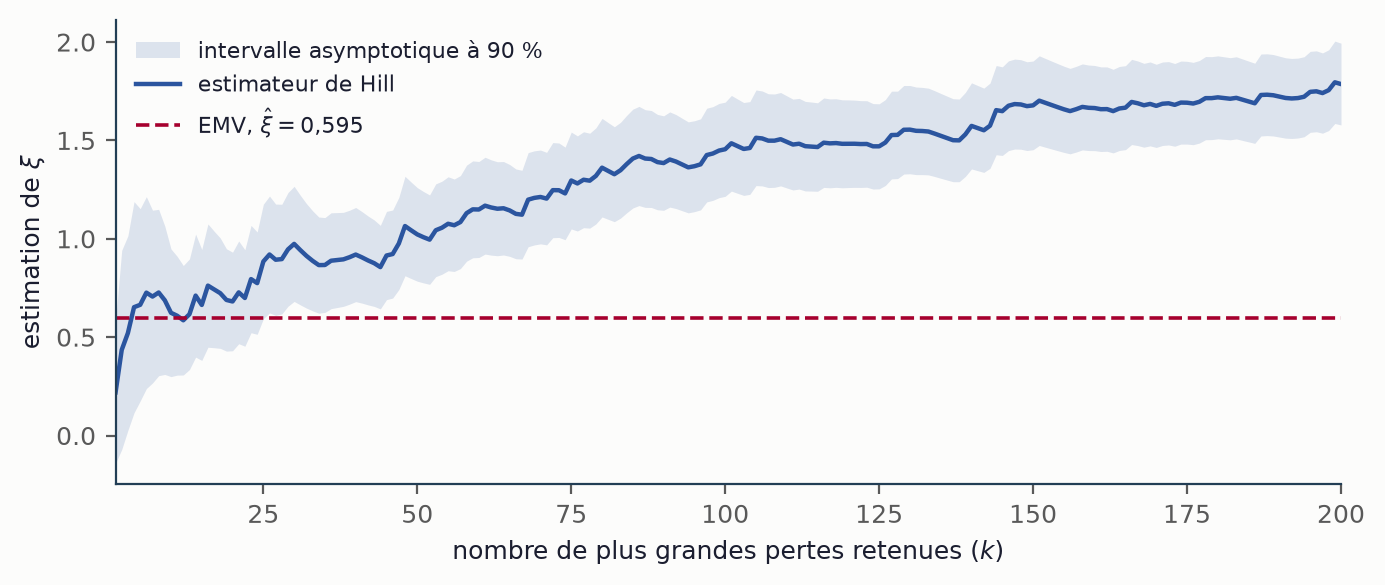
\includegraphics[width=0.85\textwidth]{hill_plot_ic90_oprisk.png}
\caption{Graphique de Hill avec intervalle de confiance asymptotique à $90\,\%$ sur OpRisk Global. La
référence du maximum de vraisemblance ($\hat{\xi} \approx 0{,}595$, pointillés rouges) n'est compatible avec
l'estimateur de Hill que pour $k \leq 25$. Au-delà, la dérive est compatible avec un biais à seuil fini,
sans suffire à en identifier la cause.}
\label{soc:fig:hill-ic}
\end{figure}

Dire que Hill est biaisé en échantillon fini est vrai en général, mais cela relève de l'argument d'autorité.
Cela ne dit pas si cet écart, sur ces données, vient du biais ou d'un désaccord réel. L'enjeu est pourtant
réel. À $\hat\xi = 0{,}595$, la variance de la sévérité est infinie mais l'espérance existe. À
$\hat\xi = 1{,}42$, l'espérance cesse d'exister, mais la perte annuelle et ses quantiles restent définis.
La simulation suivante vérifie si cet écart d'estimateurs est compatible avec le modèle retenu.

Nous simulons $2\,000$ échantillons sous le modèle publié, c'est-à-dire le corps observé sous le seuil et
une queue GPD de paramètres $(\hat\xi,\hat\sigma) = (0{,}595\,;57{,}97)$ au-dessus. Nous appliquons à chacun
le même estimateur de Hill, aux mêmes $k$. Si un monde où $\xi$ vaut $0{,}595$ reproduit les valeurs
observées, celles-ci ne prouvent rien : elles sont ce qu'un tel $\xi$ produit.

\begin{center}\footnotesize
\renewcommand{\arraystretch}{1.25}
\begin{tabular}{@{}r r r c@{}}
\toprule
$k$ & $\hat\xi_{\text{Hill}}$ observé & simulé (moyenne) & intervalle simulé à $90\,\%$ \\
\midrule
$30$  & $0{,}974$ & $0{,}835$ & $[0{,}620\,;1{,}083]$ \\
$50$  & $1{,}022$ & $0{,}987$ & $[0{,}787\,;1{,}195]$ \\
$86$  & $1{,}421$ & $1{,}423$ & $[1{,}249\,;1{,}598]$ \\
$91$  & $1{,}403$ & $1{,}405$ & $[1{,}241\,;1{,}570]$ \\
$120$ & $1{,}483$ & $1{,}484$ & $[1{,}360\,;1{,}610]$ \\
$200$ & $1{,}786$ & $1{,}787$ & $[1{,}713\,;1{,}863]$ \\
\bottomrule
\end{tabular}
\end{center}

\vspace{4pt}
\noindent Les six valeurs observées tombent dans l'intervalle simulé, et les moyennes simulées sont proches des valeurs observées, sauf pour $k=30$, où l'écart est plus net. L'écart de $138{,}6\,\%$ est donc compatible avec le modèle simulé. C'est ce que donne
Hill sur des pertes brutes, décalées du seuil, pour un échantillon de cette taille. Les données ne
contredisent pas la calibration publiée : elles lui sont compatibles par un troisième chemin, après
Anderson-Darling et Kolmogorov-Smirnov.

Ces diagnostics restent conditionnels au modèle simulé. Un plateau stable sur le tracé de Hill
serait un argument de choix du seuil, alors qu'ici l'estimateur croît sans s'arrêter, de $0{,}97$ à $k=30$ jusqu'à $1{,}79$
à $k=200$. Il monte à mesure que l'on descend dans le corps de la loi. Le balayage de seuil va dans l'autre
sens, puisque $\hat\xi$ décroît de $0{,}60$ à $0{,}51$ quand on remonte dans la queue. Ces dérives ne suffisent pas à exclure
un indice de queue de $1{,}42$ dans une autre famille compatible avec l'échantillon.

La calibration sur la PRC, par la conversion de Jacobs, donne $\hat{\xi}_{\text{PRC}} = 1{,}03$ (seuil
$u = 4{,}18$~M\euro, $2\,258$ excès), supérieur à $\hat{\xi}_{\text{OpRisk}} = 0{,}595$. Les intervalles à
$90\,\%$ ne se chevauchent pas. Un indice supérieur à un correspond à une espérance de sévérité infinie,
situation que la littérature du risque opérationnel traite explicitement \citep{neslehova2006}.

Nous posons
un plafond de sévérité de $40$~M\euro, ancré sur une capacité de réassurance cyber. Ce choix assure des
moments finis ; il n'est pas nécessaire à l'existence du quantile simulé. Ce plafond ne s'applique qu'à la PRC, la calibration OpRisk ($\xi < 1$) restant
non plafonnée. L'écart entre les deux calibrations ne mesure pas une différence de risque : la sévérité PRC
est une puissance du nombre d'enregistrements, et une puissance multiplie l'indice de queue par son exposant
(\S\ref{sec:oprisk}). Les deux sources confirment le même régime de queue lourde ($\xi > 0$). Aucune ne
prime sur l'autre, et leur écart est traité comme une composante de l'incertitude totale.

\section{Le seuil de la calibration, deux règles écrites}
\label{sec:ann-seuil}
% SOURCES-SCRIPTS: 93 47

On peut se demander pourquoi \emph{ce} seuil, et ce qu'aurait retenu une règle écrite. Nous appliquons deux
règles à dix percentiles candidats, du $70^{\text{e}}$ au $95^{\text{e}}$. La première retient le plus bas
seuil que le test d'adéquation ne rejette pas, puisque descendre gagne des excès. La seconde retient le plus
bas seuil au-dessus duquel l'indice de queue cesse de dériver, c'est-à-dire tel que tous les indices
estimés plus haut tombent dans son intervalle de confiance à $90\,\%$.

La règle de stabilité retient $19{,}32$~M\euro{} contre $20{,}03$ publiés, soit un écart de $-3{,}5\,\%$, et un
quantile supérieur de $1{,}5\,\%$ à celui qui est publié. Le seuil publié est donc voisin du plus bas
seuil au-dessus duquel $\hat\xi$ se stabilise. Cette règle fournit un contrôle rétrospectif du seuil publié ; elle n'a pas été préenregistrée avant sa calibration. Le seuil publié est aussi
le mieux ajusté du balayage, avec une $p$-value d'Anderson-Darling de $0{,}986$ contre $0{,}943$ pour le
second meilleur candidat. Deux diagnostics sur le même échantillon désignent des points voisins, ce qui n'était pas garanti.

La règle la plus permissive descendrait plus bas et donnerait davantage de capital, ce qui écarte le
soupçon d'un choix opportuniste. Elle retient $15{,}53$~M\euro, soit $22{,}5\,\%$ sous le seuil publié, où le
quantile de sévérité vaut $731{,}0$ contre $662{,}8$, soit $10{,}3\,\%$ de plus. Le seuil publié n'est donc
pas celui qui maximise le chiffre. Parmi les candidats acceptables, il est du côté qui le minore.

Sur les seuils testés, remonter réduit l'écart-type bootstrap du quantile à $99{,}5\,\%$,
de $578{,}7$ à $137{,}5$~M\euro, soit une division par $4{,}2$, alors que le nombre d'excès passe
de $171$ à $29$. Au percentile $70$, l'indice atteint $1{,}126$ : la moyenne diverge, mais pas le quantile.
Ces ajustements changent à la fois la queue estimée et l'effectif. Ils ne démontrent ni la disparition
du compromis biais-variance ni l'absence de biais au seuil le plus haut, où $29$ excès donnent une
incertitude elle-même mal connue. Le choix reste conditionnel à l'adéquation et à la stabilité.

\section{Backtest hors échantillon, détail des tests}
\label{sec:ann-backtest}
% SOURCES-SCRIPTS: 89 90 91 102

\subsection{Fréquence et forme de la queue}
% SOURCES-SCRIPTS: 89 91

La binomiale négative l'emporte sur le Poisson hors échantillon, et c'est le résultat le plus net. Les comptes annuels du périmètre ont
pour moyenne $24{,}50$ et pour variance $58{,}55$, soit un indice de dispersion de $2{,}39$, sans tendance
significative ($-0{,}092$ incident par an, $p=0{,}7297$). Une loi sans mémoire n'est donc pas mal
spécifiée sur ce point.

Sur les douze années notées, un intervalle de prévision annoncé à $90\,\%$ en couvre
$91{,}7\,\%$ sous la binomiale négative contre $75{,}0\,\%$ sous le Poisson. La couverture ne suffit pas à
trancher, puisqu'un intervalle inutilement large peut couvrir sans rien valoir. Le log-score prédictif
cumulé pénalise la largeur autant que l'étroitesse, et il désigne le même gagnant : $-41{,}334$ contre
$-44{,}388$, soit $3{,}054$ nats sur douze années. Ce résultat favorise la binomiale négative sur les douze années notées, sans mesurer
la significativité de son avantage prédictif. Il ne valide pas le facteur de dispersion posé
dans le moteur, qui reste distinct des ajustements de ce backtest.

La forme de la queue survit, et ce n'était pas acquis. Chaque ajustement d'origine ne dispose que de vingt à
quatre-vingt-dix excès. La transformée de probabilité intégrale des excès de test doit être uniforme si la loi
ajustée est la bonne. Elle a pour moyenne $0{,}532$ et le test de Kolmogorov-Smirnov ne la rejette pas
($D=0{,}100$, $p=0{,}4087$). L'écart de cette moyenne à $0{,}500$ indique des pertes qui tombent plus haut
dans la queue ajustée que prévu, mais il n'est pas significatif, et l'énoncer autrement serait
surinterpréter un test qui ne rejette pas. Ce qui est établi est plus modeste et suffit : ces données ne rejettent pas la GPD ; elles ne démontrent pas son adéquation.

\subsection{Quantiles de sévérité et dérive de l'échelle}
% SOURCES-SCRIPTS: 89 90 102

Les quantiles sont en revanche dépassés trois fois trop souvent. Sur les $280$ pertes notées, le quantile de
sévérité annoncé à $99\,\%$ par l'apprentissage est franchi huit fois pour $2{,}8$ attendues ($p=0{,}0078$), et
celui à $99{,}5\,\%$ cinq fois pour $1{,}4$ ($p=0{,}0140$). Le test de dépassement rejette donc aux deux
niveaux, là où le test de forme ne rejetait pas. Les deux constats semblent s'opposer, mais ils ne portent pas
sur le même objet. La transformée intégrale ne regarde que les excès au-dessus du seuil, donc la queue
conditionnelle, alors qu'un quantile combine la forme, le seuil et le taux de dépassement. Ce non-rejet ne localise pas à lui seul le défaut. Le taux observé change aussi : $15{,}1\,\%$ en apprentissage par
construction de la règle, $27{,}1\,\%$ hors échantillon, soit un rapport de $1{,}80$ que le test binomial situe
à $p=2{,}35\cdot 10^{-7}$. La dérive se lit aussi sur le seuil, quantile de l'apprentissage qui passe
de $8{,}56$ à $18{,}20$~M\euro{} en onze ans. La médiane annuelle des pertes monte de $13{,}0\,\%$ par
an en logarithme ($p=0{,}0003$). Ces constats motivent une échelle variable, sans exclure un défaut de famille.

Mesurer une dérive ne dit pas ce qu'elle déplace sur le nombre publié. Nous calculons cet effet sur l'échantillon
de la chaîne publiée, soit $570$ pertes dont $86$ excès au-dessus du seuil de $20{,}03$~M\euro. Un
ajustement stationnaire y donne un quantile de sévérité à $99{,}5\,\%$ de $662{,}78$~M\euro, soit la valeur
publiée.

Nous rendons ensuite l'échelle non stationnaire,
$\sigma_t = \sigma\,e^{\,b\,(t-t_{\mathrm{ref}})}$ à indice de queue constant, et l'estimons par maximum de
vraisemblance sur les mêmes excès. La dérive de la queue vaut alors $3{,}40\,\%$ par an, d'écart-type
$2{,}47\,\%$, et le rapport de vraisemblance ne la distingue pas de zéro ($1{,}81$, $p=0{,}1786$). Le quantile
évalué en fin de période passe à $774{,}73$~M\euro, soit $112$~M\euro{} et $16{,}9\,\%$ de plus. Cette estimation n'a pas
de signification statistique propre ; c'est une comparaison conditionnelle, non une borne statistique. Le taux de dépassement est tenu commun
aux deux branches ; le faire varier demanderait de réestimer conjointement la loi complète.

La dérive n'est pas la même selon l'endroit de la distribution, ce qui modère le résultat précédent. Le corps
dérive de $13{,}0\,\%$ par an quand la queue ne dérive que de $3{,}40\,\%$, soit un facteur $3{,}8$. Lire la
dérive du corps comme une dérive du capital serait donc une erreur d'un facteur voisin de quatre. La contre-épreuve
le confirme. Indexer toutes les pertes à la tendance de la médiane, puis rejouer la chaîne à
percentile de seuil constant, donne un quantile de $1\,870$~M\euro, soit $2{,}8$ fois la référence. L'indice
de queue reste sous l'unité ($0{,}68$ à la borne haute de l'intervalle de la tendance). L'hypothèse
n'est pas écartée par un argument d'existence, mais par la mesure : la dérive du corps se situe à plus de trois
écarts-types de celle de la queue.

Une part de la dérive est monétaire. Les montants de la chaîne publiée sont nominaux
(chapitre~\ref{chap:donnees}). Sur la valeur courante de la même base, qui les corrige d'une inflation
implicite de $2{,}19\,\%$ par an, la tendance de la médiane passe de $13{,}0$ à $10{,}6\,\%$ par an et reste
significative ($p=0{,}0021$). L'inflation générale n'en explique que $17\,\%$.

Dans la queue, au même seuil
publié désormais franchi par $100$ excès, la dérive passe de $3{,}40$ à $3{,}30\,\%$ par an et reste non
significative ($p=0{,}149$). L'inflation monétaire n'en explique donc qu'une faible part, et la dérive de queue ne
se distingue pas du bruit sur cet historique. Pour un capital exprimé en euros courants, le sens de l'écart
déclaré ne change pas, car une perte ancienne comptée à sa valeur nominale est sous-évaluée, que ce soit par
l'inflation ou par une aggravation du risque. Sa lecture reste prudente : la hausse de l'échelle réelle des
pertes de queue n'est pas démontrée.

Modéliser la dérive fait tomber l'indice de queue, de $0{,}5952$ à $0{,}5392$, et ce déplacement va en sens
contraire. Le mécanisme est simple : regrouper des excès d'années dont les échelles diffèrent fabrique un
mélange, et un mélange d'échelles peut faire paraître la queue plus lourde à seuil fini, sans changer nécessairement son indice asymptotique.
L'ajustement stationnaire attribue ainsi à la forme une part de ce qui relève de la dérive. Les deux écarts du
modèle publié sont de sens contraires : l'indice de queue est légèrement prudent quand l'échelle est
anti-conservatrice. Ils ne se compensent pas, puisqu'ils ne portent pas sur la même grandeur.

\subsection{Effet de la dérive sur l'écart entre états}
% SOURCES-SCRIPTS: 90

On pourrait affirmer qu'une dérive commune aux deux états de conformité se simplifie dans un rapport, donc que
l'écart DORA n'est pas concerné. L'affirmation est exacte pour une variation de la seule échelle de sévérité,
et nous l'avons mesurée. Multiplier l'échelle multiplie les deux états par le même
facteur, $1{,}3209$ en conforme contre $1{,}3166$ en non conforme, soit un rapport de $0{,}9968$ alors que les
niveaux montent de $32\,\%$. Pour cette variation, l'invariance d'échelle du facteur entre états vaut donc à
$0{,}32\,\%$ près ; multiplier toutes les pertes laisserait le facteur inchangé.

La dérive mesurée n'est pourtant pas une pure variation d'échelle. La modéliser réattribue à l'échelle ce que
l'ajustement stationnaire lisait comme de la forme, et l'indice de queue tombe de $0{,}5952$ à $0{,}5392$. Or
c'est la forme qui pèse. La composante de forme déplace seule le facteur de $-4{,}9\,\%$, soit $4{,}01$
écarts-types de simulation, alors que la composante d'échelle ne le déplace que de $-0{,}3\,\%$, sans être
résolue. Les deux sont additives, le résidu d'interaction valant $0{,}05$ écart-type. Le facteur entre états
passe ainsi de $3{,}337$ à $3{,}164$, un déplacement résolu.

L'écart en euros bouge à peine, mais par compensation et non par insensibilité. Il passe de $14\,129$ à
$13\,629$~M\euro, soit $-3{,}5\,\%$ pour un écart-type de $733$~M\euro{} entre graines, donc un déplacement non
résolu. Il serait faux d'en conclure que l'écart est robuste à la sévérité : la composante de forme seule le
ramènerait à $10\,382$~M\euro{} et celle d'échelle seule le porterait à $18\,577$. L'écart est très sensible à la
sévérité prise composante par composante, et presque insensible à la seule combinaison que produit la dérive.
Le signe et l'ordre de grandeur sont conservés dans cette variante. Le sens est favorable, puisque l'écart
comme le facteur sont plus petits sous la sévérité dérivée, le calage stationnaire donnant ici un écart plus élevé que l'ajustement
avec dérive. Le sens dépend donc de la grandeur : le niveau et l'écart entre états ne se déplacent
pas ensemble. Cette variante ne fournit aucune borne sur le capital réel.

\subsection{Charge annuelle agrégée}
% SOURCES-SCRIPTS: 91

Les tests précédents portent sur les lois marginales prises séparément, alors que le capital est le quantile de
la charge annuelle. Un modèle composé peut avoir deux marginales correctes et un agrégat faux, reproche que cette
classe de modèles reçoit le plus souvent. L'observable noté est la somme annuelle des sinistres dépassant le
seuil d'apprentissage, qui est l'objet que produit la chaîne publiée puisqu'elle donne une sévérité nulle sous le
seuil. La prédictive est obtenue par $200\,000$ années simulées à chaque origine. Le verdict est négatif. La
transformée intégrale de l'agrégat vaut $0{,}734$ en moyenne pour $0{,}500$ attendu, et Kolmogorov-Smirnov la
rejette ($D = 0{,}484$, $p = 0{,}0042$). L'intervalle de prévision annoncé à $90\,\%$ n'en couvre que $75{,}0\,\%$,
avec trois dépassements de sa borne haute concentrés dans les quatre dernières années notées.

Ce rejet est compatible avec une dérive, sans exclure d'autres défauts de spécification. Une dérive laisse une
signature reconnaissable, puisqu'elle ne désaligne pas les premières années notées mais seulement les dernières,
l'apprentissage prenant du retard à mesure qu'elle s'accumule. La mesure le montre : la transformée intégrale vaut
$0{,}611$ sur les six premières années notées contre $0{,}857$ sur les six dernières, un écart que le test de
Mann-Whitney situe à $p = 0{,}0130$. La charge observée passe en moyenne de $363$ à $1\,255$~M\euro{} entre les deux
moitiés, quand la médiane prédictive ne passe que de $183$ à $248$. Aucune limite nouvelle ne s'ajoute donc à
l'inventaire du chapitre~\ref{ch:robustesse}. La même s'y lit plus fort, l'agrégat cumulant la dérive de l'échelle
et celle du taux de dépassement, quand chaque marginale n'en portait qu'une.

L'avantage de la binomiale négative sur les comptes se retrouve peu sur la charge annuelle.
Notée au score de probabilité continu classé
sur la charge agrégée, son avance sur le Poisson tombe à $0{,}3\,\%$. La charge annuelle est portée par un sinistre
unique, donc par la queue de sévérité et non par la surdispersion du comptage. La binomiale négative reste le bon
choix, mais elle n'est plus un déterminant du niveau de capital et il ne faut pas la présenter ainsi.

Reste l'indépendance entre fréquence et sévérité. Le modèle composé retenu la suppose ; des modèles composés dépendants existent aussi.
Une dépendance positive pourrait modifier la queue de l'agrégat. Sur l'ensemble de la distribution, la
régression du logarithme du montant d'un sinistre sur le nombre d'incidents de son année donne une pente négative
et significative, $-0{,}02397$ à $p = 0{,}0419$. Une tendance linéaire en année y est contrôlée pour ne pas confondre l'effet avec
la dérive. Sur les seuls excès, qui sont la population que le modèle tire, cette pente tombe à $-0{,}00331$ et cesse
d'être significative ($p = 0{,}84$), soit $0{,}14$ de sa valeur. Cette différence est compatible avec un effet de profondeur de collecte : une année à beaucoup d'incidents enregistrés est une année où l'on
descend plus bas, et non une propriété du risque. Prise au pied de la lettre sur les excès, sa conséquence sur le
quantile de l'agrégat est de l'ordre du pour cent et symétrique en signe. Les corrélations de rang entre le compte
annuel et la médiane ou le maximum de l'année ne rejettent rien non plus. Le rang est ici le bon outil : à
$\hat\xi$ voisin de $0{,}6$, la variance de la sévérité est infinie, si bien qu'un test adossé à la variance de
l'agrégat n'aurait pas d'objet.
